\documentclass[11pt]{article}

\usepackage{fancyhdr}
\usepackage{extramarks}
\usepackage{amsmath}
\usepackage{amsthm}
\usepackage{amsfonts}
\usepackage{bm}
\usepackage{tikz}
\usepackage{graphicx}
\usepackage{float}
\usepackage{enumerate}
\usepackage{hyperref}

\usetikzlibrary{positioning, arrows}
\tikzstyle{int}=[draw, fill=blue!20, minimum size=4em]
\tikzstyle{init} = [pin edge={to-,thin,black}]

%
% Basic Document Settings
%
\hypersetup{
    colorlinks=true,
    linkcolor=magenta,
    filecolor=magenta,      
    urlcolor=blue,
    pdftitle={Jaydev Singh Rao (19147): Planar VTOL Design Study}
    }

\topmargin=-0.45in
\evensidemargin=0in
\oddsidemargin=0in
\textwidth=6.5in
\textheight=9.0in
\headsep=0.25in

\linespread{1.1}

\pagestyle{fancy}
\lhead{\tiny{\hmwkAuthorName \space \hmwkAuthorRoll}}
\rhead{\tiny{\hmwkClass \ (\projecttitle)}}
\cfoot{\tiny\thepage}

\renewcommand\headrulewidth{0.4pt}
\renewcommand\footrulewidth{0.4pt}

\setlength\parindent{0pt}

\setcounter{secnumdepth}{0}
\newcounter{objectivecounter}
\setcounter{objectivecounter}{1}
\nobreak\extramarks{Objective \arabic{objectivecounter}}{}\nobreak{}

\newenvironment{Objective}[1]{
    \section{\arabic{objectivecounter}. #1}
    \stepcounter{objectivecounter}
}{}

\newcommand{\projecttitle}{Planar VTOL System}
\newcommand{\hmwkTitle}{Design Study}
\newcommand{\hmwkClass}{ECS 323: Control Systems}
\newcommand{\hmwkAuthorName}{Jaydev Singh Rao}
\newcommand{\hmwkAuthorRoll}{19147}

%
% Title Page
%

\title{
    \vspace{1in}
    \hrule
    \vspace{0.25in}
    \textmd{\textbf{\Huge \hmwkClass}}\\
    \vspace{1in}
    \textmd{\textbf{\Huge \projecttitle}} \\
    \vspace{0.1in}\normalsize{\textmd{\LARGE \hmwkTitle}}\\
    \vspace{1in}
    \normalsize\vspace{0.1in}\LARGE{Submitted by: \hmwkAuthorName}\\
    \normalsize\vspace{0.1in}\LARGE{Roll No. : \hmwkAuthorRoll}
}

\author{}
\date{}

%
% Various Helper Commands
%

% For derivatives
\newcommand{\de}[2]{\cfrac{\mathrm{d}#1}{\mathrm{d}#2}}

% For partial derivatives
\newcommand{\pde}[2]{\cfrac{\partial #1}{\partial #2}}

%integral
\newcommand{\integrate}[4]{\displaystyle \int_{#3}^{#4} #1 \mathrm{d}#2}

% Integral dx
\newcommand{\dx}{\mathrm{d}x}

% Alias for the Solution section header
\newcommand{\solution}{\textbf{\large Solution}}

% Centered figure
\newcommand{\centerfig}[4][0.35]{
    \begin{figure}[H]
        \centering
        \fbox{\includegraphics[scale=#1]{#2}}
        \caption{#3}
        \label{fig:#4}
    \end{figure}
    }

\begin{document}

    \maketitle
    \hrule
    \pagebreak
    \tableofcontents
    \pagebreak

    \begin{Objective}{Design Study Description}
        In this design study we need to design a control system for a planar VTOL system with the given parameters \cite{controlbook}:
        \begin{itemize}
            \item $M_c=2 \text{ kg}$
            \item $J_c = 0.009 \text{ kg m$^2$}$
            \item $m_l = 0.3 \text{ kg}$
            \item $m_r = 0.3 \text{ kg}$
            \item $d = 0.28 \text{ m}$
            \item $\mu = 0.21 \text{ kg s$^{-1}$}$
        \end{itemize}
        \centerfig[0.5]{./planar_vtol_diagram.png}{Planar VTOL System}{vtol_fig}
    \end{Objective}

    \pagebreak

    \begin{Objective}{Kinetic Energy}
        The postions of the various components of the VTOL are given by:
        \[ 
            \begin{split}
                \mathbf{p_c} & = (z_v,\ h) \\
                \mathbf{p_l} & = (z_v - d \cos\theta,\ h - d \sin\theta) \\
                \mathbf{p_r} & = (z_v + d \cos\theta,\ h + d \sin\theta)
            \end{split}    
        \]
        So, the velocities can be written as:
        \[ 
            \begin{split}
                \mathbf{v_c} & = (\dot z_v,\ \dot h) \\
                \mathbf{v_l} & = (\dot z_v + d\dot \theta \sin\theta,\ \dot h - d \dot \theta \cos\theta) \\
                \mathbf{v_r} & = (\dot z_v - d \dot \theta \sin \theta,\ \dot h + d \dot \theta \cos \theta)
            \end{split}    
        \]

        Kinetic energy of the centerpod is given by:
        \begin{equation}
            \label{KE_pod}
            K_{pod} = \frac12 m_c \mathbf{v}_c^T \mathbf{v}_c + \frac12 \bm{\omega}_c^TJ_c \bm{\omega}_c = \frac12 m_c (\dot z_v^2 + \dot h^2) + \frac12 J_c \dot \theta ^2
        \end{equation}

        Kinetic energy of the left and right rotors is given by:
        \begin{equation}
            \label{KE_rotors}
            \begin{split}
                K_{rotors} & = \frac12 m_l \mathbf{v}_l^T \mathbf{v}_l + \frac12 m_r \mathbf{v}_r^T \mathbf{v}_r \\
                    & = \frac12 m_l (\dot z_v + d\dot \theta \sin\theta)^2 + \frac12 m_l (\dot h - d \dot \theta \cos\theta)^2 \\
                    & \quad + \frac12 m_r (\dot z_v - d\dot \theta \sin\theta)^2 + \frac12 m_l (\dot h + d \dot \theta \cos\theta)^2 \\
                    & = \frac12 (m_l + m_r) (\dot z_v^2 + \dot h^2) + \frac12 (m_l + m_r) d^2 \dot \theta^2 \\
                    & \quad + (m_l-m_r)(\dot z_v \sin \theta - \dot h \cos \theta) d\dot \theta
            \end{split}
        \end{equation}

        Now, the total kinetic energy of the VTOL will be given by the sum of (\ref{KE_pod}) and (\ref{KE_rotors}):
        \begin{equation}
            \label{KE_vtol}
            \begin{split}
                K_{V} & = K_{pod} + K_{rotors} \\
                & = \frac12 (m_c + m_l + m_r) (\dot z_v^2 + \dot h^2) + \frac12 (m_l d^2 + m_r d^2 + J_c) \dot\theta^2 \\
                & \quad\quad + (m_ld - m_rd)(\dot z_v \sin \theta - \dot h \cos \theta) \dot \theta
            \end{split}
        \end{equation}

        As in the given parameters $m_l = m_r$, so the last term in the kinetic energy is zero and will be ignored in the rest of the report.
    \end{Objective}

    \pagebreak

    \begin{Objective}{Equations of Motion}
        \begin{enumerate}[(a)]
            \item Now in order to determine the equations of motion of the VTOL, we first write its potential energy. The potential energy is due to the gravitational potential and can be written as the sum of potential energies of the individual components:
            \begin{equation}
                \label{PE_vtol}
                P_V = m_c g h + m_l g h + m_r g h = (m_c + m_l + m_r) g h
            \end{equation}

            \item Now as we are only considering the dynamics of the VTOL and not of the target so the generalized coordinates can be defined as:
            \[\mathbf q = \begin{pmatrix}
                z_v \\ h \\ \theta
            \end{pmatrix}\]

            Also as it is given in the project objective, the damping forces in the system are due to the momentum drag which is caused by the change in direction of the air when it flows through the rotors. This momentum drag can be modeled as $F_{drag} = -\mu \dot z_v$. So, we can write the dissipative (drag) forces as:
            \[- B\mathbf{\dot q} = - \begin{pmatrix}
                \mu \dot z_v \\ 0 \\ 0
            \end{pmatrix} = - \begin{pmatrix}
                \mu & 0 & 0 \\ 0 & 0 & 0 \\ 0 & 0 & 0
            \end{pmatrix} \begin{pmatrix}
                \dot z_v \\ \dot h \\ \dot \theta
            \end{pmatrix}\]

            \item The total force on the COM of the VTOL is given by $\boxed{F = f_l + f_r}$. The torque due to the left rotor is $\tau_l = - f_l d$ (using right handed coordinates) and the torque due to the right rotor is $\tau_r = f_r d$. Hence, the total torque about the COM of the VTOL is $\boxed{\tau = (f_r - f_l) d}$. So, we can write the generalized forces as:
            \[\bm\Phi = \begin{pmatrix}
                - F \sin \theta \\ F \cos \theta \\ \tau
            \end{pmatrix} = \begin{pmatrix}
                - (f_r + f_l) \sin \theta \\ (f_r + f_l) \cos \theta \\ (fr - f_l) d
            \end{pmatrix}\]

            \item Using the kinetic and the potential energies (\ref{KE_vtol}) and (\ref{PE_vtol}) we can write the Lagrangian as:
            \[
                \begin{split}
                    \mathcal{L} & = K_V - P_V = \frac12 M_V (\dot z_v^2 + \dot h^2 - 2gh) + \frac12 J_V \dot\theta^2
                \end{split}
            \]
            Here, $M_V \equiv (m_c + m_l + m_r)$ and $J_V \equiv (m_l d^2 + m_r d^2 + J_c)$. Now, we can write:
            \[
                \pde{\mathcal L}{\mathbf{\dot q}} = \begin{pmatrix}
                    M_V\dot z_v \\ M_V \dot h \\ J_V \dot\theta
                \end{pmatrix}
            \]

            And,
            \[
                \pde{\mathcal L}{\mathbf{q}} = \begin{pmatrix}
                    0 \\ - M_V g \\ 0
                \end{pmatrix} 
            \]

            Writing the Euler-Lagrange equations in matrix form:
            \[
                \de{}{t}\biggl(\pde{\mathcal L}{\mathbf{\dot q}}\biggr) - \pde{\mathcal L}{\mathbf{q}} = \bm \Phi - B\mathbf{\dot q}
            \]
            \[
                \implies \begin{pmatrix}
                    M_V\ddot z_v \\ M_V \ddot h \\ J_V \ddot\theta
                \end{pmatrix} - \begin{pmatrix}
                    0 \\ - M_V g \\ 0
                \end{pmatrix} = \begin{pmatrix}
                    - F \sin \theta \\ F \cos \theta \\ \tau
                \end{pmatrix} - \begin{pmatrix}
                    \mu \dot z_v \\ 0 \\ 0
                \end{pmatrix}
            \]
            \begin{equation}
                \label{EOM_vtol}
                \implies
                \boxed{
                    \begin{pmatrix}
                        M_V\ddot z_v \\ M_V \ddot h \\ J_V \ddot\theta
                    \end{pmatrix} = \begin{pmatrix}
                        - \mu \dot z_v - F \sin \theta \\ - M_V g + F \cos \theta \\ \tau
                    \end{pmatrix}
                }
            \end{equation}
        \end{enumerate}
    \end{Objective}

    \pagebreak

    \begin{Objective}{Linearize Equations of Motion}
        \begin{enumerate}[(a)]
            \item First we determine the equilibrium points of the equations of motion (\ref{EOM_vtol}) of the VTOL. At this point there is no motion in the system. This means:
            \[\mathbf{\dot q} = \begin{pmatrix}
                \dot z_v \\ \dot h \\ \dot \theta
            \end{pmatrix} = \begin{pmatrix}
                0 \\ 0 \\ 0
            \end{pmatrix}\]

            And consequently,
            \[\mathbf{\ddot q} = 0 \implies \begin{pmatrix}
                M_V\ddot z_v \\ M_V \ddot h \\ J_V \ddot\theta
            \end{pmatrix} = 0\]

            \[ \begin{pmatrix}
                - \mu \dot z_v - F \sin \theta \\ M_V g + F \cos \theta \\ \tau
            \end{pmatrix} = 0 \implies \begin{pmatrix}
                - F \sin \theta \\ - M_V g + F \cos \theta \\ \tau
            \end{pmatrix} = 0\]

            The solutions of the above equations are given by, $\theta_e = 0$ or $\theta_e = \pi$ and due to this $F_e =  M_V g$ or $F_2 = -M_V g$ and $\tau_e = 0$. The values of $z_e$ and $h_e$ can be anything.
            
            But taking the practical consideration that the rotors are able to rotate in only one direction the case where $\theta = \pi$ and $F_e = - M_V g$, the rotors can not generate a positive force in the opposite direction of the direction of lift. So, we will drop this case.

            \item In order to linearize the equations, we first write the equations seperately in the form:
            \[\begin{split}
                \ddot z_v & = - \frac{\mu}{M_V}\dot z_v - \frac{F}{M_V} \sin\theta\\
                \ddot h & = - g + \frac{F}{M_V}\cos \theta \\
                \ddot \theta & = \frac{1}{J_c}\tau
            \end{split}\]

            Now, we define:
            \[
                \tilde{z} \equiv z_v - z_v^{(e)},\ \tilde{h} \equiv h - h_e,\ \tilde{\theta} \equiv \theta - \theta_e,\ \tilde F \equiv F - F_e,\ \tilde \tau \equiv \tau - \tau_e = \tau
            \]

            Also, we can note that as $\mathbf{\dot q}_e = 0$ and $\mathbf{\ddot q}_e = 0$, so we can write:
            \[\dot{\tilde z} = \dot z_v,\ \ddot{\tilde z} = \ddot z_v\]
            \[\dot{\tilde h} = \dot h,\ \ddot{\tilde h} = \ddot h\] 
            \[\dot{\tilde \theta} = \dot \theta,\ \ddot{\tilde \theta} = \ddot \theta\]

            Now we linearize the non-linear terms in these equations as follows:
            \[
                \begin{split}
                    \frac{\mu}{M_V}\dot z_v & \approx \frac{\mu}{M_V}\dot z_v^{(e)} + \pde{}{\dot z_v}\bigg(\frac{\mu}{M_V}\dot z_v\bigg) \bigg\rvert_{eq.} (\dot z_v - \dot z_v^{(e)}) \\
                    & = \frac{\mu}{M_V}\dot{\tilde z} \\
                    \frac{F}{M_V} \sin\theta & \approx \frac{F}{M_V} \sin\theta_e + \pde{}{\theta}\bigg(\frac{F}{M_V} \sin\theta\bigg) \bigg\rvert_{eq.} (\theta - \theta_e) \\
                    & = \frac{F_e}{M_V} \tilde\theta\cos\theta_e \\
                    & = g \tilde\theta \\
                    \frac{F}{M_V} \cos\theta & \approx \frac{F}{M_V} \cos\theta_e + \pde{}{\theta}\bigg(\frac{F}{M_V} \cos\theta\bigg) \bigg\rvert_{eq.} (\theta - \theta_e) \\
                    & = \frac{F}{M_V} +  \frac{F_e}{M_V}\tilde\theta\sin\theta_e \\
                    & = \frac{F}{M_V} \\
                    & = \frac{\tilde F}{M_V} + g
                \end{split}
            \]

            So, the linearized equations of motion are:
            \begin{equation}
                \label{EOM_vtol_linear}
                \begin{split}
                    \ddot{\tilde z} & = - \frac{\mu}{M_V}\dot{\tilde z} - g\tilde\theta \\
                    \ddot{\tilde h} & = \frac{\tilde F}{M_V}\\
                    \ddot{\tilde\theta} & = \frac{1}{J_c}\tilde\tau
                \end{split}
            \end{equation}

            \item The equations of motion can only be feedback linearized if we can write the equations in the from given below where $y(t)$ is the output and $u(t)$ is the input with the function $g(y, \dot y)$ giving the non-linear terms.
            \[a\ddot y + b\dot y + cy = g(y,\dot y) + u(t)\]

            But in the case of the equations of motion of the planar VTOL given by (\ref{EOM_vtol}), the non-linerity is present in the input term itself ($F$ is the input), and hence we can't seperately define $g(y,\dot y)$. Hence, the system can not be feedback linearized. 

        \end{enumerate}
    \end{Objective}

    \pagebreak

    \begin{Objective}{Transfer Function Model}
        \begin{enumerate}[(a)]
            \item We have the linearized equations of motion given in (\ref{EOM_vtol_linear}). If we take the laplace transform of those equations we get the following:
            \[\begin{split}
                s^2 \tilde Z(s) & = - \frac{\mu}{M_V} s \tilde Z(s) - g\tilde \Theta(s) \\
                s^2 \tilde H(s) & = \frac{1}{M_V} \tilde{F}(s) \\
                s^2 \tilde \Theta(s) & = \frac{1}{J_c} \tilde{\tau}(s)
            \end{split}\]

            \item For longitudinal dynamics we have the following equation:
            \[ 
                \begin{split}
                    & s^2 \tilde H(s) = \frac{1}{M_V} \tilde{F}(s) \\
                    \implies &  \boxed{\tilde H(s) = \frac{1}{s^2 M_V} \tilde{F}(s)}
                \end{split}
            \]

            Hence, in the longitudinal dynamics we have $\tilde F(s)$ as the input variable and $\tilde H(s)$ as the output with transfer function $\frac{1}{s^2 M_V}$.

            \item For lateral dynamics first we have the equation for $\tilde \Theta (s)$:
            \[
                \begin{split}
                    & s^2 \tilde \Theta(s) = \frac{1}{J_c} \tilde{\tau}(s) \\
                    \implies & \boxed{\tilde\Theta(s) = \frac{1}{s^2 J_c} \tilde{\tau}(s)}
                \end{split}  
            \]

            And, also we have the equation for $\tilde Z(s)$ given by:
            \[
                \begin{split}
                    & s^2 \tilde Z(s) = - \frac{\mu}{M_V} s \tilde Z(s) - g\tilde \Theta(s) \\
                    \implies & \tilde Z(s) + \frac{\mu}{s M_V}\tilde Z(s) = - \frac{g}{s^4 J_c} \tilde{\tau}(s) \\
                    \implies & \tilde Z(s) = - \frac{\frac{g}{s^4 J_c} \tilde{\tau}(s)}{1 + \frac{\mu}{s M_V}} \\
                    \implies & \boxed{\tilde Z(s) = - \frac{M_V g}{s^3 J_c (sM_V + \mu)}\tilde\tau(s)}
                \end{split}    
            \]

            Hence, in the lateral dynamics we have $\tilde{\tau}(s)$ is the input variable, $\tilde{\Theta}(s)$ is the intermediate variable with transfer function \( \frac{1}{s^2 J_c} \) and $\tilde{Z}(s)$ is the output variable with transfer function \(- \frac{M_V g}{s^3 J_c (sM_V + \mu)}\).

            \pagebreak

            \item The block diagrams of open loop longitudinal and lateral systems are:
            
            \vspace{0.5in}

            \begin{figure}[H]
                \centering
                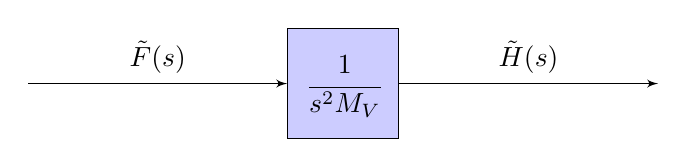
\begin{tikzpicture}[node distance=2.5cm,auto, > = latex']
                    \node [int] (a) {$\cfrac{1}{s^2 M_V}$};
                    \node (b) [left of=a,node distance=4cm, coordinate] {$\tilde F(s)$};
                    \node (c) [right of=a,node distance=4cm, coordinate] {$\tilde H(s)$};
                    \node [coordinate] (end) [right of=c, node distance=4cm]{};
                    \path[->] (b) edge node {$\tilde F(s)$} (a);
                    \path[->] (a) edge node {$\tilde H(s)$} (c);
                \end{tikzpicture}
                \caption{Longitudinal open loop system}
                \label{fig:long_ol_diagram}
            \end{figure}

            \vspace{0.5in}

            \begin{figure}[H]
                \centering
                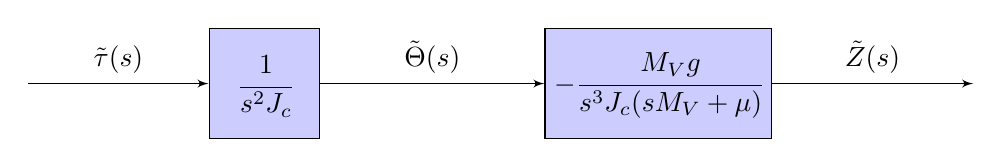
\begin{tikzpicture}[node distance=2.5cm,auto, > = latex']
                    \node [int, minimum size=4em] (a) {$\cfrac{1}{s^2 J_c}$};
                    \node (b) [left of=a,node distance=3cm, coordinate] {$\tilde \tau(s)$};
                    \node [right of=a, minimum size=2.5em, node distance=5cm, int] (c) {$- \cfrac{M_V g}{s^3 J_c (sM_V + \mu)}$};
                    \node [coordinate] (end) [right of=c, node distance=4cm]{};
                    \path[->] (b) edge node {$\tilde \tau(s)$} (a);
                    \path[->] (a) edge node {$\tilde \Theta(s)$} (c);
                    \path[->] (c) edge node {$\tilde Z(s)$} (end);
                \end{tikzpicture}
                \caption{Lateral open loop system}
                \label{fig: lat_ol_diagram}
            \end{figure}
        \end{enumerate}
        
    \end{Objective}

    \pagebreak

    \begin{Objective}{State Space Model}
        \begin{enumerate}[(a)]
            \item For the longitudinal dynamics we define the state of the system as \( \tilde x_{lon} = \begin{pmatrix} \tilde h & \dot{\tilde h} \end{pmatrix}^{\mathrm T}\), the input as \(\tilde u_{lon} = \tilde F\) and the output as \(\tilde y_{lon} = \tilde h\). Now we can write:
            \[
                \begin{split}
                    & \dot{\tilde x}_{lon} = \begin{pmatrix}
                        \dot{\tilde{h}} \\ \ddot{\tilde{h}}
                    \end{pmatrix} = \begin{pmatrix}
                        \dot{\tilde{h}} \\ \frac{\tilde F}{M_V}
                    \end{pmatrix} \\
                    \implies & \dot{\tilde x}_{lon} = \begin{pmatrix}
                        \dot{\tilde{h}} \\ \frac{\tilde u_{lon}}{M_V}
                    \end{pmatrix} = \begin{pmatrix}
                        0 & 1 \\ 0 & 0
                    \end{pmatrix} \begin{pmatrix}
                        \tilde h \\ \dot{\tilde{h}}
                    \end{pmatrix} + \begin{pmatrix}
                        0 \\ \frac1{M_V}
                    \end{pmatrix} \tilde{u}_{lon} \\
                    \implies & \dot{\tilde x}_{lon} = A \tilde x_{lon} + B \tilde{u}_{lon} \\
                \end{split}
            \]

            Similary for the output we have:
            \[
                \begin{split}
                    & \tilde y_{lon} = \tilde h \\
                    \implies & \tilde y_{lon} = \begin{pmatrix} 1 & 0 \end{pmatrix} \begin{pmatrix}
                    \tilde h \\ \dot{\tilde h} \end{pmatrix} + \begin{pmatrix} 0 \end{pmatrix} \tilde{u}_{lon} \\
                    \implies & \tilde y_{lon} = C \tilde x_{lon} + D \tilde u_{lon}
                \end{split}  
            \]

            \item For the lateral dynamics we define the state as \(\tilde x_{lat} = \begin{pmatrix}
                \tilde z & \tilde\theta & \dot{\tilde z} & \dot{\tilde \theta}
            \end{pmatrix}^{\mathrm T}\) with the input \(\tilde u_{lat} = \tilde{\tau}\) and output \(\tilde y_{lat} = \begin{pmatrix} \tilde z & \tilde \theta \end{pmatrix}^{\mathrm T}\). So for this we have:

            \[
                \begin{split}
                    & \dot{\tilde{x}}_{lat} = \begin{pmatrix}
                        \dot{\tilde z} \\ \dot{\tilde\theta} \\ \ddot{\tilde z} \\ \ddot{\tilde \theta}
                    \end{pmatrix} = \begin{pmatrix}
                        \dot{\tilde z} \\ \dot{\tilde\theta} \\ - \frac{\mu}{M_V}\dot{\tilde z} - g\tilde\theta \\ \frac{1}{J_c}\tilde\tau
                    \end{pmatrix} \\
                    \implies & \dot{\tilde{x}}_{lat} = \begin{pmatrix}
                        0 & 0 & 1 & 0 \\
                        0 & 0 & 0 & 1 \\
                        0 & - g & - \frac{\mu}{M_V} & 0 \\
                        0 & 0 & 0 & 0
                    \end{pmatrix} \begin{pmatrix}
                        \tilde z \\ \tilde\theta \\ \dot{\tilde z} \\ \dot{\tilde \theta}
                    \end{pmatrix} + \begin{pmatrix}
                        0 \\ 0 \\ 0 \\ \frac{1}{J_c}
                    \end{pmatrix} \tilde{\tau} \\
                    \implies & \dot{\tilde{x}}_{lat} = A \tilde{x}_{lat} + B \tilde{u}_{lat}
                \end{split}    
            \]

            Similary, for the output we have:

            \[\begin{split}
                & \tilde y_{lat} = \begin{pmatrix}
                    \tilde z \\ \tilde \theta
                \end{pmatrix} = \begin{pmatrix}
                    1 & 0 & 0 & 0 \\
                    0 & 1 & 0 & 0
                \end{pmatrix} \begin{pmatrix}
                    \tilde z \\ \tilde\theta \\ \dot{\tilde z} \\ \dot{\tilde \theta}
                \end{pmatrix} + \begin{pmatrix}
                    0
                \end{pmatrix} \tilde \tau \\
                \implies & \tilde y_{lat} = C \tilde{x}_{lat} + D \tilde{u}_{lat}
            \end{split}\]
        \end{enumerate}
    \end{Objective}

    \pagebreak

    \begin{thebibliography}{1}
        \bibitem{controlbook} Randal W Beard, Timothy W. McLain, Cammy Peterson, Marc Killpack (2021), ``Introduction to Feedback Control using Design Studies'', \url{http://controlbook.byu.edu/doku.php}
    \end{thebibliography}

\end{document}